Последовательный метод SOR~\eqref{eq:sor_update} не допускает параллелизма: обновление каждого узла зависит от значений, вычисленных для соседних узлов на той же итерации. Современные GPU содержат тысячи вычислительных ядер и эффективны при одновременном выполнении большого числа независимых операций. Для использования этого потенциала необходимо переформулировать итерационный процесс так, чтобы обновления узлов на каждом шаге были независимы. Шахматная (Red-Black) раскраска сетки позволяет достичь этого: на каждом полуходе обновляются узлы только одного цвета, и их обновления не зависят друг от друга. Полученный метод Red-Black SOR сохраняет сходимость классического SOR, но допускает массово-параллельную реализацию.

\textit{Шахматная раскраска сетки.}
Каждому узлу~$(i,\,j)$ присваивается цвет в зависимости от чётности суммы индексов:
\begin{equation}\label{eq:rb_coloring}
  c(i,j) = (i + j) \bmod 2.
\end{equation}

Схема шахматной раскраски в~сравнении с~последовательным обходом
при~обычном SOR приведена на~рисунке~\ref{fig:rb_coloring}.

\begin{figure}[!ht]
\centering
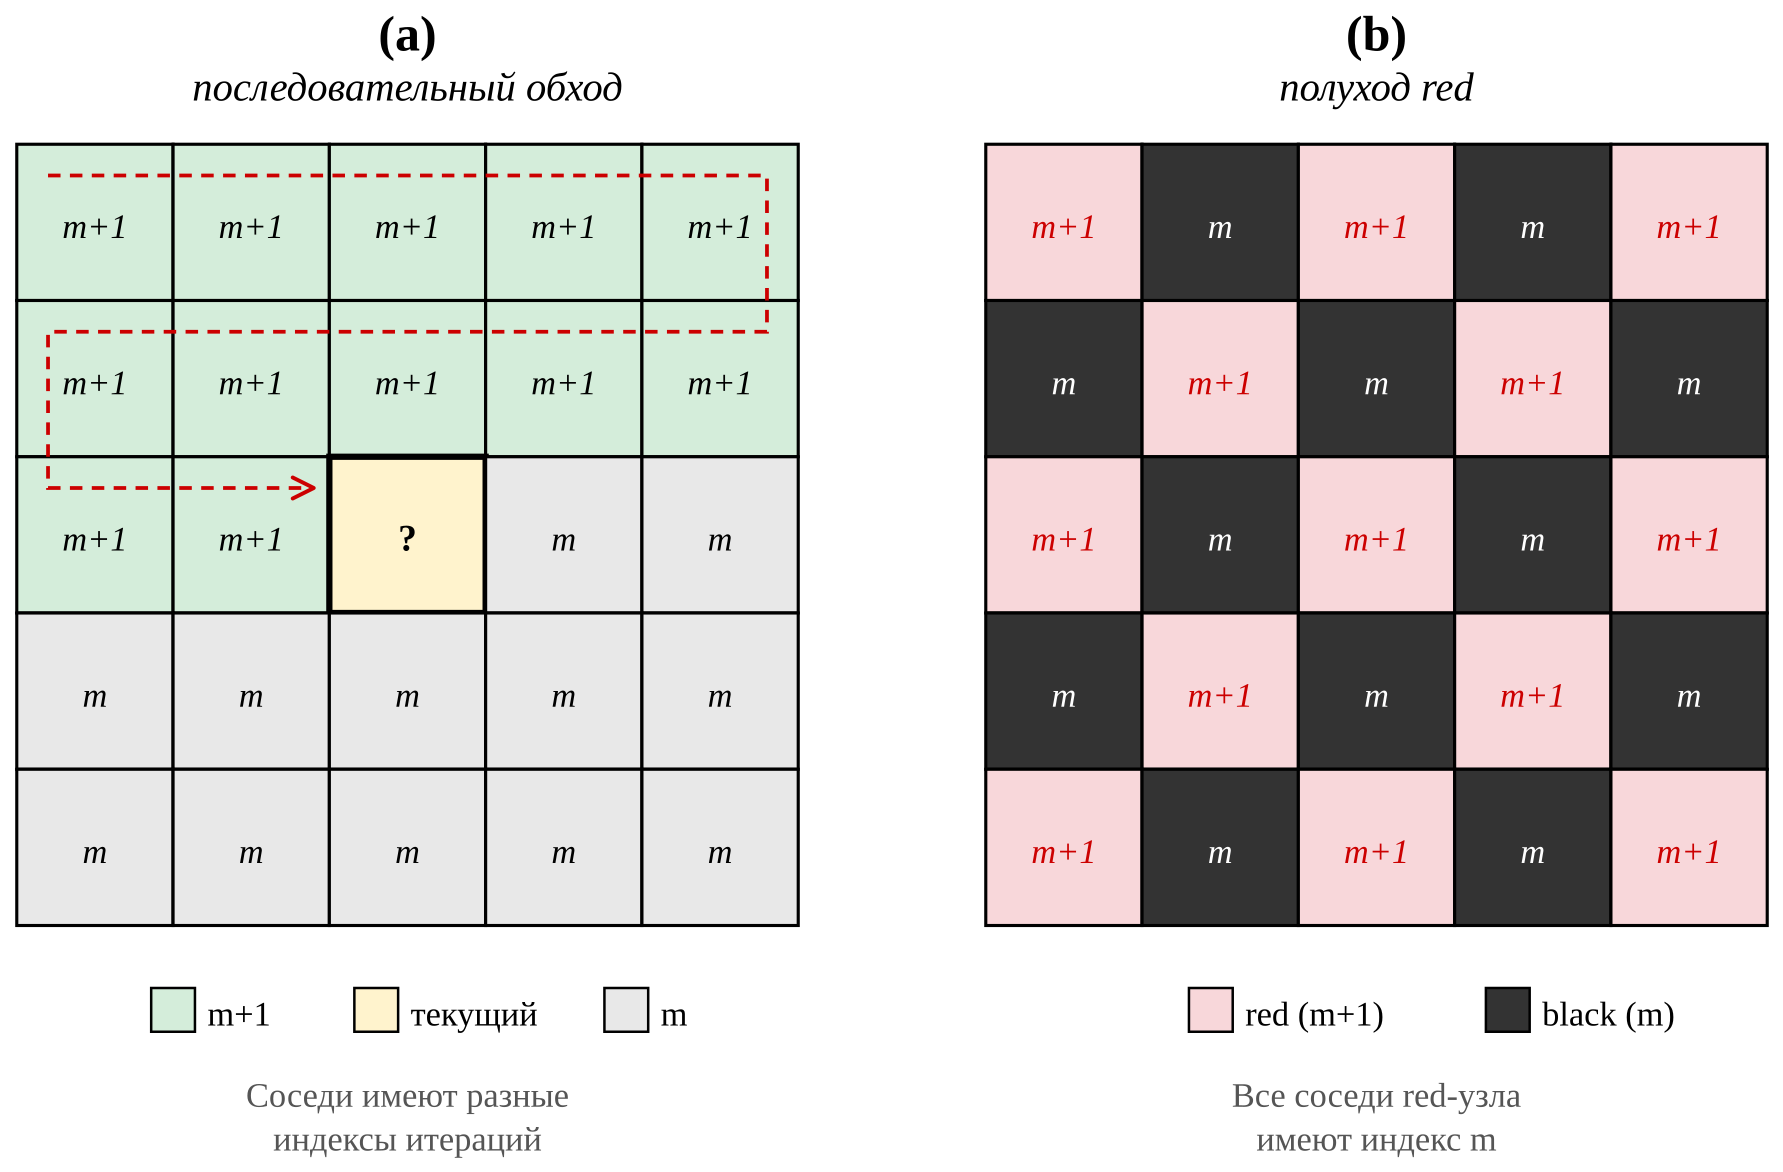
\includegraphics[width=\textwidth,height=0.9\textheight,keepaspectratio]{figures/ch03/fig_3_2.png}
\caption{Сравнение обхода сетки при обычном SOR и шахматной (Red--Black)
раскраске: (а)~последовательный обход по строкам смешивает индексы
итераций; (б)~полуход red обновляет только красные узлы, чёрные соседи
сохраняют индекс~$m$, что обеспечивает независимость обновлений}
\label{fig:rb_coloring}
\end{figure}

\FloatBarrier

Узлы с~$c = 0$ (условно «красные») и~$c = 1$ («чёрные») образуют два непересекающихся подмножества, покрывающих всю сетку. Название связано с аналогией шахматной доски: красные узлы занимают клетки одного цвета, чёрные~-- другого. Ключевое свойство раскраски состоит в том, что в пятиточечном шаблоне~\eqref{eq:5point_stencil} каждый красный узел имеет только чёрных соседей и наоборот. Поэтому при одновременном обновлении всех красных узлов каждый из них использует только значения чёрных соседей, которые не менялись на текущем полуходе,~-- все соседи имеют единый итерационный индекс (на полуходе red~-- индекс~$(m)$, на полуходе black~-- индекс~$(m+\tfrac{1}{2})$, см.\ формулы~\eqref{eq:rb_sor_red}-\eqref{eq:rb_sor_black}). Это свойство делает обновления внутри одного цвета полностью независимыми друг от друга и пригодными для массово-параллельного выполнения: каждый узел может обновляться отдельным потоком GPU без синхронизации с другими потоками. Синхронизация требуется только между полуходами и обеспечивается последовательным запуском ядер GPU: завершение ядра red гарантирует видимость обновлённых значений для ядра black (внутри одного ядра межпоточная синхронизация не требуется). Два полухода составляют одну полную итерацию.

\textit{Обновление давления на полуходе.}
В отличие от классического SOR~\eqref{eq:sor_update}, где часть соседних значений уже обновлена на текущей итерации (индексы~$(m)$ и~$(m+1)$ перемешаны), в Red-Black варианте обновление выполняется в два полухода с чёткой индексацией. На полуходе red обновляются узлы цвета~$c = 0$; их соседи (цвет~$c = 1$) сохраняют значения с итерации~$m$:
\begin{equation}\label{eq:rb_sor_red}
\begin{split}
  &\tilde{p}_{i,j} = \frac{1}{a_P}\bigl(
    a_E\,p_{i+1,j}^{(m)} + a_W\,p_{i-1,j}^{(m)}
    + a_N\,p_{i,j+1}^{(m)} + a_S\,p_{i,j-1}^{(m)}
    + b_{i,j}\bigr), \\
  &p_{i,j}^{(m+1/2)} = p_{i,j}^{(m)}
    + \omega\bigl(\tilde{p}_{i,j} - p_{i,j}^{(m)}\bigr),
    \qquad c(i,j) = 0.
\end{split}
\end{equation}

На полуходе black обновляются узлы цвета~$c = 1$; их соседи (цвет~$c = 0$) уже обновлены на текущей итерации и имеют индекс~$(m+1/2)$:
\begin{equation}\label{eq:rb_sor_black}
\begin{split}
  &\tilde{p}_{i,j} = \frac{1}{a_P}\bigl(
    a_E\,p_{i+1,j}^{(m+1/2)} + a_W\,p_{i-1,j}^{(m+1/2)} + \\
  &+ a_N\,p_{i,j+1}^{(m+1/2)} + a_S\,p_{i,j-1}^{(m+1/2)}
    + b_{i,j}\bigr), \\
  &p_{i,j}^{(m+1)} = p_{i,j}^{(m)}
    + \omega\bigl(\tilde{p}_{i,j} - p_{i,j}^{(m)}\bigr),
    \qquad c(i,j) = 1.
\end{split}
\end{equation}

Внутри каждого полухода все соседи имеют фиксированные значения (противоположный цвет не обновляется), что обеспечивает полную независимость обновлений и пригодность для массово-параллельного выполнения на GPU. Заметим, что на полуходе black релаксация в~\eqref{eq:rb_sor_black} выполняется от~$p_{i,j}^{(m)}$, поскольку чёрные узлы не затрагивались на полуходе red. В ядре обновления при необходимости выполняется проекция~$p \leftarrow \max(p,\, p_{\mathrm{cav}})$. В расчётах в избыточных давлениях обычно~$p_{\mathrm{cav}} = 0$. Проекция используется в режимах расчёта с кавитацией (условие Гюмбеля (half-Sommerfeld), раздел~3.5); в режиме полного заполнения может быть отключена.

\textit{Граничные условия на GPU.}
После каждой полной итерации (полуход red, затем полуход black) выполняется отдельное ядро, применяющее граничные условия из раздела~3.1. Внутренние узлы расположены в диапазоне~$i = 1, \ldots, N_z - 2$, $j = 1, \ldots, N_\varphi - 2$; слои~$j = 0$ и~$j = N_\varphi - 1$ используются как ghost-узлы для реализации периодичности, а строки~$i = 0$ и~$i = N_z - 1$ соответствуют торцевым границам с условиями Дирихле. Периодичность по окружному направлению обеспечивается копированием значений в ghost-узлы на границах: $P[i,\,0] = P[i,\,N_\varphi-2]$, $P[i,\,N_\varphi-1] = P[i,\,1]$. Это гарантирует корректное обращение к соседям при следующем полуходе. Условия Дирихле на торцах по оси~$z$ реализуются установкой давления кавитации: $P[0,\,j] = p_{\mathrm{cav}}$, $P[N_z-1,\,j] = p_{\mathrm{cav}}$. Граничные условия вынесены в отдельное ядро, чтобы не усложнять ветвление в основном ядре обновления. Это также упрощает адаптацию к другим типам граничных условий (например, при расчёте сектора вместо полного кольца). Ядро граничных условий запускается с одномерной сеткой потоков: каждый поток обрабатывает одну строку (для периодичности) или один столбец (для Дирихле).

\textit{Организация вычислений и конфигурация запуска.}
Ядро обновления давления использует двумерную сетку потоков GPU. Блок потоков имеет размер~$32 \times 8$: 32~потока по быстрому (окружному) индексу~$j$ соответствуют одной warp-линии~-- группе потоков, выполняющихся синхронно на одном мультипроцессоре. Такой выбор обеспечивает коалесцированный (последовательный) доступ к глобальной памяти: соседние потоки обращаются к соседним элементам массива, что минимизирует число транзакций памяти. Размер сетки блоков вычисляется из числа внутренних узлов: $(N_\varphi - 2)$ по окружному и $(N_z - 2)$ по осевому направлению. Потоки, попадающие за пределы расчётной области, завершаются без выполнения операций.

Каждый поток обрабатывает один внутренний узел. Поток вычисляет свои индексы~$(i,\,j)$ и проверяет условие раскраски~$c(i,j) = (i+j) \bmod 2$. Если цвет узла не совпадает с текущим полуходом, поток пропускает обновление. Все данные (давление, коэффициенты, правая часть) хранятся в глобальной памяти GPU в формате двойной точности. Коэффициенты дискретизации предварительно вычисляются на GPU из поля зазора~$h$ средствами поэлементных операций.

Ядро граничных условий запускается с одномерной сеткой потоков (блок из 256~потоков). Размер сетки определяется максимумом из~$N_z$ и~$N_\varphi$. Каждый поток обрабатывает либо одну строку (копирование для периодичности), либо один столбец (обнуление для Дирихле).

Коэффициенты дискретизации в реализации обозначаются~$A$, $B$, $C$, $D$, $E$, $F$ и связаны с обозначениями раздела~3.2 соотношениями: $A = a_E$, $B = a_W$, $C = a_N$, $D = a_S$, $E = a_P$, $F = b_{i,j}$.

\textit{Контроль сходимости.}
Сходимость контролируется по критерию относительной поправки~\eqref{eq:convergence_change} из раздела~3.3. Для снижения накладных расходов проверка выполняется не на каждой итерации, а с интервалом (типично~-- каждые несколько сотен итераций, таблица~\ref{tab:solver_params}). Перед началом блока итераций сохраняется копия текущего поля давления в отдельный GPU-буфер. После завершения блока вычисляется~$\delta^{(m)}$ средствами массовых операций GPU: поэлементное вычитание массивов, суммирование модулей разностей и суммирование модулей текущего решения. Эти операции выполняются на GPU без переноса данных на CPU; на CPU передаётся только скалярный результат~$\delta^{(m)}$. При $\delta^{(m)} < \varepsilon$ итерации прекращаются.

Проверка сходимости не на каждой итерации обусловлена тем, что вычисление~$\delta$ требует глобальной редукции (суммирования по всему массиву), которая является синхронной операцией и нарушает конвейер GPU. Выполнение редукции каждые несколько сотен итераций (а не каждую) практически не влияет на точность определения момента сходимости, но существенно снижает накладные расходы.

\textit{Кэширование GPU-буферов.}
При решении серии задач на одной сетке (например, параметрическое варьирование эксцентриситета, угла наклона, глубины микрорельефа) размер массивов не меняется. Выделение и освобождение GPU-памяти~-- дорогостоящие операции; повторное их выполнение на каждом вызове решателя создаёт значительные накладные расходы. Поэтому при первом вызове для данного размера сетки~$N_z \times N_\varphi$ выделяются рабочие буферы (массивы давления, копии для проверки сходимости, массивы коэффициентов дискретизации). При последующих вызовах с тем же размером сетки буферы переиспользуются~-- выполняется только обнуление массива давления и пересчёт коэффициентов. Это особенно эффективно при расчёте характеристик подшипника в диапазоне параметров, когда решатель вызывается десятки и сотни раз подряд.

\textit{Алгоритм итерации.}
На вход подаётся поле зазора~$h_{i,j}$, шаги сетки~$\Delta x_1$, $\Delta x_2$ и геометрические параметры ($R$,~$L$). На первом этапе из поля зазора вычисляются коэффициенты дискретизации~$a_E$, $a_W$, $a_N$, $a_S$, $a_P$ и правая часть~$b_{i,j}$~-- все операции выполняются на GPU. Поле давления инициализируется нулями.

Далее выполняется итерационный цикл. Одна полная итерация состоит из трёх этапов: обновление давления в узлах цвета~$c = 0$ (полуход red), обновление в узлах цвета~$c = 1$ (полуход black), применение граничных условий. С заданным интервалом (типично каждые 500~итераций) перед блоком итераций сохраняется копия поля давления, а после блока вычисляется относительная поправка~$\delta^{(m)}$~\eqref{eq:convergence_change}. Если $\delta^{(m)} < \varepsilon$, итерации прекращаются. Если достигнуто максимальное число итераций, процесс также останавливается с фиксацией достигнутого значения~$\delta$.

По завершении итераций результирующее поле давления переносится из памяти GPU на CPU для дальнейшего вычисления интегральных характеристик (несущая способность, момент трения, утечки; см.\ подраздел <<Целевые функционалы и выходные величины>>)~\cite{ansys2013}.

Описанный GPU-решатель применяется как внутренний решатель линейной системы в алгоритме JFO (раздел~3.5), где дополнительно выполняется обновление активного множества и вычисление степени заполнения~$\vartheta$ в кавитационной зоне.
